\documentclass[../../../../Assignments.tex]{subfiles}

% \documentclass{book}
% \usepackage{pgfplots}
% \pgfplotsset{compat=1.17}


\begin{document}
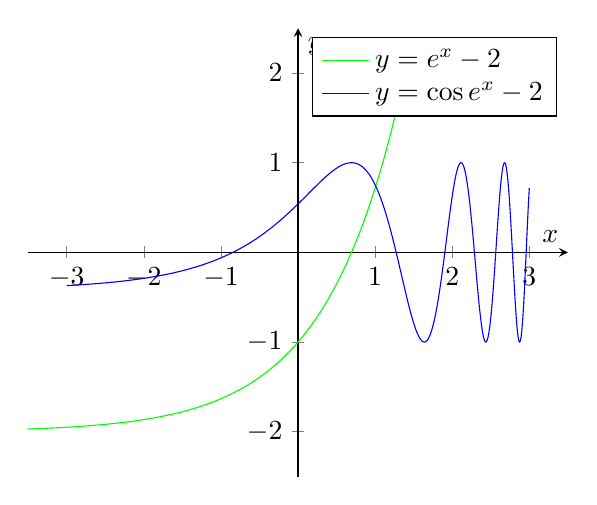
\begin{tikzpicture}
    \begin{axis}[
        axis lines=center,
        samples=1000,
        xlabel={\(x\)},
        xmin=-3.5,xmax=3.5,
        ylabel={\(y\)},
        ymin=-2.5,ymax=2.5,
        legend cell align={left},
    ]
        \addplot [green, restrict y to domain=-2:2] {e^x - 2};
        \addlegendentry{\(y = e^x - 2\)}

        \addplot [blue, domain=-3:3] {cos(deg(e^x - 2))};
        \addlegendentry{\(y = \cos{e^x - 2}\)}
    \end{axis}
\end{tikzpicture}
\end{document}
